\documentclass{standalone}
\usepackage{tikz}
\usepackage{amsmath,amssymb}
\begin{document}
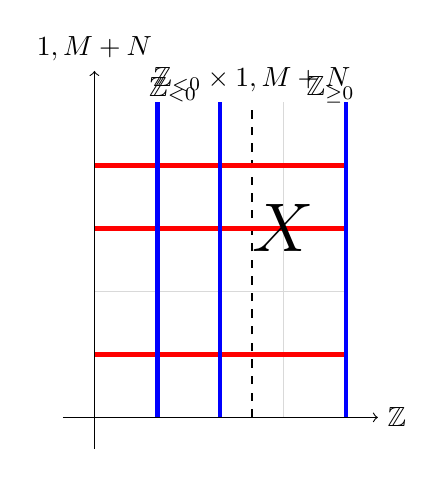
\begin{tikzpicture}[scale=0.8]
  % Grid lines
  \foreach \x in {0,1,2,3,4} {
    \draw[gray!30] (\x,0) -- (\x,5);
    \draw[gray!30] (0,\x) -- (4,\x);
  }
  
  % Vertical dashed line
  \draw[dashed, thick] (2.5,0) -- (2.5,5) node[above] {$\mathbb{Z}_{< 0} \times \llbracket 1, M + N \rrbracket$};
  
  % Colored lines (original cross moved)
  \foreach \y in {1,3,4} {
    \draw[red, line width=1.5pt] (0,\y) -- (2.5,\y);
    \draw[red, line width=1.5pt] (2.5,\y) -- (4,\y);
  }
  \foreach \x in {1,2,4} {
    \draw[blue, line width=1.5pt] (\x,0) -- (\x,2.5);
    \draw[blue, line width=1.5pt] (\x,2.5) -- (\x,5);
  }
  
  % Cross symbol at moved position
  \node at (3,3) {\Huge $X$};
  
  % Axis labels
  \draw[->] (-0.5,0) -- (4.5,0) node[right] {$\mathbb{Z}$};
  \draw[->] (0,-0.5) -- (0,5.5) node[above] {$\llbracket 1, M + N \rrbracket$};
  
  % Region labels
  \node at (1.25,5.2) {$\mathbb{Z}_{< 0}$};
  \node at (3.75,5.2) {$\mathbb{Z}_{\geq 0}$};
\end{tikzpicture}
\caption{Vertex configuration from \Cref{fg3} after applying the Yang-Baxter equation to relocate the crossing to the right of $\mathbb{Z}_{< 0} \times \llbracket 1, M + N \rrbracket$.}
\end{document}